\section{Metsandus}
Metsad omavad olulist rolli nii ühiskonna igapäevaelus kui ka planeedi heaolus.
Alates mööblis kasutatavast puidust kuni paberini, millele kirjutame. Lisaks neile
nähtavatele toodetele sisaldavad paljud ravimid, kosmeetika ja pesuvahendid
metsadest saadud kõrvalsaadusi. Rohkem kui 1,6 miljardit inimest sõltub
metsadest toidu ja kütuse saamisest ning umbes 70 miljonit, sealhulgas paljud
põlisrahvad, peavad metsi oma koduks \cite{karsentyUnderlyingCausesRapid2003}. 
Metsad varustavad meid hapnikuga, pakuvad
varjualust, töökohti, puhast vett ja toitu, olles seega inimkonna ellujäämiseks
hädavajalikud. Kuna nii paljude inimeste elu sõltub metsadest, on metsade saatus
otseselt seotud ka meie endi tulevikuga. \cite{WWFImportanceForests} 

\section{Copernicus ja EstHub}
Copernicus on üks osa Euroopa kosmoseprogrammist (EUS), mis tegeleb planeedi jälgimisega. Copernicus programmi raames, lisaks maa pealse info kogumisele, on loodud mitmeid satelliite, mis koguvad informatsiooni kosomosest. See info on kõigile kättesaadav tasuta. Selle programmiga seotud satellite kutsutakse \textbf{Sentineliks}. \cite{CopernicusCopernicus}


EstHub on Eesti riiklik satelliitandmete keskus, mis kogub ja integreerib
mitmekesiseid georuumilisi andmeid automatiseeritud protsesside kaudu.
Andmekogumine hõlmab kõrge resolutsiooniga satelliitkaadrite allalaadimist ja
standardiseerimist erinevatest allikatest. EstHubi eesmärk on koguda kokku sateliidi andmed mis katavad Eesti territooriumi. \cite{maa-ametNationalSatelliteData}

\begin{figure}[H]
    \centering
    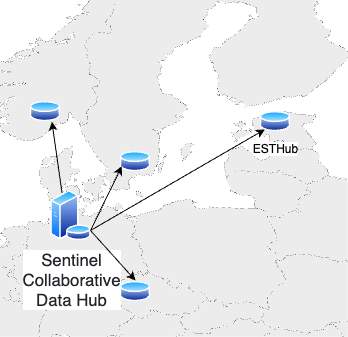
\includegraphics[width=.3\textwidth]{figures/datahubEU.drawio.png}
    \caption{Sateliidi andmete liikumine andmekeskuste vahel}
    \label{fig:esthubliiklus}
\end{figure}


\subsection{Sentinel}
Sentinel-1 on radaripõhine satelliit, mis võimaldab jälgida maapinna vajumist,
struktuuride kahjustusi ning looduskatastroofe nagu maavärinad ja maalihked. Samuti on
see ideaalne mere- ja Arktika seireks, sealhulgas laevade jälgimiseks ning
naftareostuse tuvastamiseks. \cite{S1Applications}

Sentinel-2 missioon koosneb kahest identsest satelliidist, Sentinel-2B
(käivitatud 2017) ja Sentinel-2C (käivitatud 2024), mis töötavad koos, et
pakkuda kõrge eraldusvõimega multispektraalseid pilte Maa pindadest,
rannikualadest ja siseveekogudest iga viie päeva järel. Need andmed toetavad
rakendusi põllumajanduses, metsanduses ja maakatte klassifitseerimisel. \cite{S2Applications}

Sentinel-3 on Euroopa Maa seire satelliitmissioon, mille eesmärk on mõõta
merepinna topograafiat, mere ja maa pinnatemperatuure ning ookeani ja maa
pinnavärvi suure täpsusega. Neid andmeid kasutatakse ookeani prognoosisüsteemides,
keskkonnaseires ja kliimaseires. \cite{S3Mission}

Sentinel-5P on esimene Copernicuse missioon, mis on pühendatud atmosfääri
seirele. See kannab tipptasemel \textbf{Tropomi} instrumenti, mis kaardistab mitmeid
gaase nagu lämmastikdioksiid, osoon, formaldehüüd, vääveldioksiid, metaan,
vingugaas ja aerosoolid - kõik need mõjutavad meie hingatavat õhku, tervist ja
kliimat. \cite{S5PApplications}
\subsection{Lainepikkuste spekter}
Spektriribad on satelliitandmete analüüsimisel üliolulised, sest need
võimaldavad eristada maapinna erinevaid omadusi, lähtudes elektromagnetilise
spektri konkreetsetest lainepikkustest. Näiteks Sentinel-2 MSI instrumendi 13
spektririba hõlmavad nähtavat valgust, lähedast infrapunat ja lühilaine
infrapunat, võimaldades detailset maastiku klassifitseerimist, sealhulgas
metsade, veekogude ja muu loodusliku keskkonna eristamist. Iga ribaga seondub
kindel lainepikkuse vahemik, mida spetsiifiliste filtrite abil eraldatakse. \cite{S2Mission}
\bigskip

\begin{longtable}{llll}
    \hline
    Riba & Resolutsioon & Kasutus                          \\ 
    \hline
    B01  & 60$m \mkern3mu px^{-1}$        & Aerosool                         \\
    B02  & 10$m \mkern3mu px^{-1}$        & Sinine                           \\
    B03  & 10$m \mkern3mu px^{-1}$        & Roheline                         \\
    B04  & 10$m \mkern3mu px^{-1}$        & Punane                           \\
    B05  & 20$m \mkern3mu px^{-1}$        & Vegetatsiooni klassifitseerimine \\
    B06  & 20$m \mkern3mu px^{-1}$        & Vegetatsiooni klassifitseerimine \\
    B07  & 20$m \mkern3mu px^{-1}$        & Vegetatsiooni klassifitseerimine \\
    B08  & 10$m \mkern3mu px^{-1}$        & Lähiinfrapunariba on hea rannajoonte ja biomassisisalduse kaardistamiseks \\
    B8A  & 20$m \mkern3mu px^{-1}$        & Kitsam lähedane infrapunane  \\
    B09  & 60$m \mkern3mu px^{-1}$        & Veeaur tuvastus                       \\
    B10  & 60$m \mkern3mu px^{-1}$        & Pilvede tuvastus                      \\
    B11  & 20$m \mkern3mu px^{-1}$        & Lühilaine infrapunane 1      \\
    B12  & 20$m \mkern3mu px^{-1}$        & Lühilaine infrapunane 2      \\
         &              &                    &                              \\ \hline
    \caption{Sentinel-2 MSI spektriribad ja nende kasutusvaldkonnad}
    \label{tab:s2bands}
\end{longtable}

\subsection{Koordinaatsüsteemid ja CRS}
Koordinaatsüsteem on meetod, mille abil määratletakse ja kirjeldatakse punktide
asukohti maastikul, kasutades koordinaate. Selles kontekstis eristatakse kahte
tüüpi: geograafilised koordinaatsüsteemid, mis kasutavad laiuse ja pikkuse
väärtusi, ning projekteeritud koordinaatsüsteemid, mis teisendavad
geograafilised koordinaadid lameda kaardi koordinaatideks, kasutades
matemaatilisi projektsioone. CRS ehk koordinaatide viite süsteem määratleb
reeglid ja parameetrid, mille alusel need koordinaadid seonduvad reaalse
maastikuga. \cite{8CoordinateReference}

\section{Masinõppe meetodite kasutus kaugseires}
smt smt smt smt smt
